\chapter{Inferenz und Resolution}
\label{chap:inferenz_resolution}

\section{Inferenz}
\label{sec:inferenz}
Sofern nicht anders vermerkt, basiert der folgende Abschnitt auf~\cite[S. 163 - 165]{russel}.

Grundsätzlich geht es bei Inferenz um den Prozess von Schlussfolgerungen mit Hilfe von Resolution (siehe~\ref{sec:resolution}). Die logische Inferenz ist ein Prozess der Inferenz und der Resolution, welcher die Folgebeziehungen zwischen Sätzen zum Ausdruck bringt.

\subsection{Inferenz in Computern}
\label{subsec:inferenz-in-computer}

Das grundsätzliche Problem bei Computern im Bezug auf Inferenz ist, dass ein Computer keine Interpretation vornehmen kann und nichts über die (Um-) Welt weiss, bzw.\ nur, was in seiner Wissensdatenbank gespeichert ist.


Angenommen, man möchte einen Computer fragen:

\lstset{caption={Beispielanfrage an eine Wissensdatenbank eines Computers},captionpos=b}
\begin{lstlisting}
    ``Ist eine Abenteuerreise eine Reise?''
\end{lstlisting}

so weiss der Computer weder was ein Abenteuerreise ist, noch kennt er das Konzept des Reisens an sich. Das Einzige, was er tun kann, ist in der Wissensdatenbank zu suchen nach:

\lstset{caption={Aussage in einer Wissensdatenbank eines Computers},captionpos=b}
\begin{lstlisting}
    ``Eine Abenteuerreise ist eine Reise.''
\end{lstlisting}

Findet der Computer diese Aussage in der Wissensdatenbank, so spielt es keine Rolle, dass er das Konzept der Abenteuerreise oder des Reisens nicht kennt. Die Schlussfolgerung, dass eine Abenteuerreise eine Reise ist, trifft unter allen Gegebenheiten und Interpretationen zu, welche für die Wissensdatenbank zutreffen.

Zusammenfassend ist die formale Inferenz in der Lage, gültige Schlussfolgerungen zu ziehen, auch wenn der Computer die Interpretationen des Anwenders nicht kennt. Der Computer zieht immer logisch gültige Schlüsse, unabhängig von der (menschlichen) Interpretation. Da der Mensch in der Regel die Interpretation kennt, erscheinen die Schlüsse dem Menschen logisch.

\section{Resolution}
\label{sec:resolution}
Sofern nicht anders vermerkt, basiert der folgende Abschnitt auf~\cite[S. 277 - 279]{russel}.

Resolution, aus dem Lateinischen ``resolutio'', zu Deutsch ``Auflösung'', ist eine Verallgemeinerung des Modus Ponens. Der Modus Ponens ``\ldots stellt eine universelle Schlussregel dar, die unabhängig vom jeweiligen Problem angewandt werden kann.''~\cite[S. 41]{laemmel} Beispiel: \textit{Regen = nasse Strasse. Regen gegeben, also muss die Strasse nass sein.}

Die Methode der Resolution wurde 1965 von J. A. Robinson entwickelt. Dabei handelt es sich um einen vollständigen Algorithmus des Theorembeweises für Prädikatenlogik erster Stufe.~\cite[S. 18]{russel} In der einfachsten Form der Resolution handelt es sich um eine Inferenz-Regel der Aussagenlogik.

Eine Verallgemeinerung der einfachen Form der Inferenz-Regel zur Resolution kann als Regel zur kompletten Inferenz der Prädikatenlogik erster Stufe genutzt werden.

\section{Inferenz und Resolution zur Ziehung von Schlüssen}
\label{sec:inferenz_praktisch}
Inferenz in der Semantik kann grundsätzlich als das Entdecken von neuen Beziehungen zwischen Entitäten beschrieben werden. Das bedeutet, automatische Prozeduren, in Form von so genannten \textit{Reasonern}, leiten neue Beziehungen ab. Wie  die neuen Beziehungen generiert werden, ist eine Frage der Implementation, z.B. durch Hinzufügen zu den vorhandenen Daten oder durch einfache Rückgabe derselben (vgl.~\cite[Abschn. 1]{w3inference}).

Reasoner sind Komponenten, welche eine Folgerung von implizitem Wissen zulassen bzw.\ anbieten. Es handelt sich um eine Art ``Verstehen'' der Maschinen. Ziel ist es, aus explizitem Wissen in Form einer Ontologie implizites Wissen zu gewinnen.

Eine detaillierte Beschreibung, wie man einen Reasoner in der Praxis umsetzt, findet sich in Form des \textit{Pellet}-Reasoners der Firma Clark \& Parsia im~\autoref{sec:inferenz_pellet}. Der \textit{Pellet}-Reasoner basiert auf Beschreibungslogik.  Eine Einführung der Grundlagen der Beschreibungslogik folgt im nächsten Abschnitt.

\subsection{Beschreibungslogik}
\label{subsubsection:beschreibungslogik}
Beschreibungslogiken sind Formalismen um Wissen darzustellen. Sie sind dabei eine Teilmenge der Prädikatenlogik und stellen den Kern von Wissensrepräsentationssystemen dar.
Sie sind eine Struktur für eine Wissensbasis und den damit verbundenen Methoden zur semantischen Folgerung (vgl.~\cite{dl:baader2003}) von neuem Wissen aus der Wissensbasis.

Die Struktur, welche Beschreibungslogiken als Wissensbasis bereitstellt, besteht aus einem Schema (Tbox, Regeln) und aus Daten (Abox, Fakten).

Details zu Beschreibungslogiken finden sich unter~\cite{dl:baader2003}.

\subsubsection{Interpretation}
\label{subsubsection:beschreibungslogik_Interpretation}
``Man bezeichnet die Zuordnung von Ereignissen aus einer realen Welt zu aussagenlogischen Variablen als Interpretation.''~\cite[S. 36]{laemmel}

\begin{lstlisting}[caption={Definition einer Interpretation \protect\footnotemark}]
    Sei M die Menge aller aussagenlogischen Formeln. Eine Funktion
        $I : M \rightarrow \{ W , F \}$
    heisst Interpretation.
\end{lstlisting}
\footnotetext{\cite[S. 36]{laemmel}}

\subsubsection{Modell}
\label{subsubsection:beschreibungslogik_modell}
\begin{lstlisting}[caption={Definition Modell \protect\footnotemark}]
    Sei $I$ eine Interpretation und $X$ eine aussagenlogische Formel.
    Ist $X$ unter $I$ wahr, so bezeichnet man $I$ als Modell von $X$.
\end{lstlisting}
\footnotetext{\cite[S. 37]{laemmel}}

\subsubsection{Semantische Folgerung}
\label{subsubsection:beschreibungslogik_semfol}
``Der Zusammenhang von Formeln kann durch den Begriff der semantischen Folgerung dargestellt werden.''~\cite[S. 39]{laemmel}

\begin{lstlisting}[caption={Definition semantische Folgerung\protect\footnotemark}]
    Sei $X$ eine Menge von aussagenlogischen Formeln, $Y$ eine aussagenlogische Formel.
        $Y$ ist eine semantische Folgerung von $X$
    falls jedes Modell von $X$ auch Modell von $Y$ ist.
    Man schreibt dafür $X \models Y$ und sagt auch $Y$ folgt aus $X$.
\end{lstlisting}
\footnotetext{\cite[S. 39]{laemmel}}

\subsubsection{Ableitbarkeit}
\label{subsubsection:beschreibungslogik_ableitbarkeit}
Es ist erforderlich, ``\dots dass das Folgern von Formeln auf der Ebene der Gültigkeit von der Berechnung von Formeln auf der Inferenzebene unterschieden wird. Dies wird mit dem Begriff des Ableitens getan.''~\cite[S. 42]{laemmel}

\begin{lstlisting}[caption={Definition Ableitbarkeit\protect\footnotemark}]
    $Y$ ist aus $X$ ableitbar,
        $X \vdash Y$
    wenn eine endliche Folge von Inferenzschritten existiert,
    so dass man von $X$ zu $Y$ gelangt.
\end{lstlisting}
\footnotetext{\cite[S. 42]{laemmel}}

\subsubsection{Korrektheit und Vollständigkeit}
\label{subsubsection:beschreibungslogik_vollstanendigkeit}
``Der Bezug zwischen beiden Begriffen (semantische Folgerung und Ableitbarkeit, Anm.\ der Autoren) wird durch die Begriffe der Korrektheit und der Vollständigkeit hergestellt.''~\cite[S. 43]{laemmel}

\begin{lstlisting}[caption={Definition Korrektheit und Vollständigkeit\protect\footnotemark}]
    Ein Beweis-Verfahren heisst korrekt, wenn für beliebige Formeln $X, Y$ gilt:
        Falls $X \vdash Y$ gilt, dann gilt auch $X \models Y$.
    Ein Beweis-Verfahren heißt vollständig, wenn für beliebige Formeln $X, Y$ gilt:
        Falls $X \models Y$ gilt, dann gilt auch $X \vdash Y$.
\end{lstlisting}
\footnotetext{\cite[S. 43]{laemmel}}

\subsubsection{Äquivalenz von semantischer Folgerung und Widerspruchsbeweis}
\label{subsubsection:beschreibungslogik_widersp}
Um zu überprüfen, ob eine Formel wahr ist, kann getestet werden, ob Ihre Negation falsch ist. Es wird also ein Widerspruchsbeweis durchgeführt.
~\cite[vgl. S. 47]{laemmel}

\begin{lstlisting}[caption={Äquivalenz von semantischer Folgerung und Widerspruchsbeweis}]
		Folgende Aussagen sind äquivalent:
				X $X \models Y$ Y
		X $\land$ $\lnot$ Y ist widersprüchlich
\end{lstlisting}
\footnotetext{\cite[S. 47]{laemmel}}


\section{Pellet}
\label{sec:inferenz_pellet}
Sofern im Text nicht anders vermerkt, basiert das nachfolgende Kapitel auf~\cite{sirin:pellet05}.

Bei Pellet handelt es sich um einen Reasoner auf Basis von Beschreibungslogik. OWL ist eine syntaktische Variante der Beschreibungslogik.\@ Bei der Entwickelung von Pellet wurde von Anfang an nur die OWL-DL~\footnote{\url{http://www.w3.org/TR/owl-ref/\#OWLDL}}-Sprache berücksichtigt. Diese ist wiederum eine Teilsprache von OWL-full, siehe~\autoref{chap:owl}.

Eine komplette Unterstützung des OWL-full Profils ist generell nicht möglich, da dieses nicht entscheidbar ist. Daher beschränkt sich Pellet auf die Verwendung von OWL-DL\@.~\cite[S. 13]{sirin:pellet05}

\begin{figure}[htbp]
\centering \rotatebox{0}{\scalebox{0.5}[0.5]{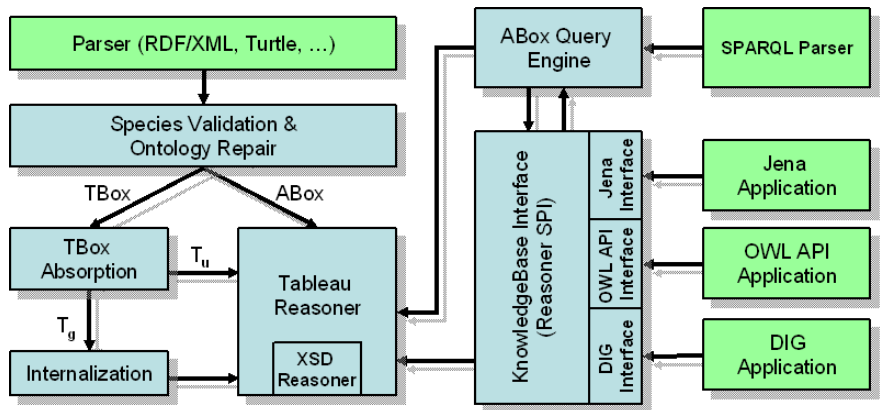
\includegraphics{bilder/pellet_komponenten.png}}}
\caption{Hauptkomponenten des Pellet-Reasoners.\label{fig:pellet_komponenten}\protect\footnotemark}
\end{figure}
\footnotetext{\cite[S. 6]{sirin:pellet05}}

Die obenstehende Abbildung zeigt die Hauptkomponenten von Pellet. Dabei ist der Tableau-Reasoner die Kernkomponente, welche die Wissensbasis auf deren Konsistenz prüft. Der Entscheid bei der Entwicklung von Pellet, ausschliesslich OWL-DL zu verwenden, führte zu einer modularen Struktur. Module ihrerseits sind z.B.\ ein Reasoner zur Datentypenprüfung eines XML-Schemas oder eine ``Query-Engine''. Genaueres dazu wird in den nachfolgenden Abschnitten beschrieben.

Hier eine Übersicht der wichtigsten Komponenten von Pellet\cite[S. 4]{sirin:pellet05}:
\begin{table}[H]
\centering
\fbox{\begin{minipage}[t]{0.48\linewidth}%
    \begin{tabbing}
        Abkürzung \= Bezeichnung ******** \= Beschreibung \kill \\
        ---           \> Tableau-Reasoner  \> Komponente, zum Ziehen von Schlüssen durch Konsistenzprüfung \\
                      \>                    \> einer Ontolgie.  \\
        \textbf{Abox} \> Assertional Box    \> Komponente, welche Aussagen zu Individuen enthält, \\
                      \>                    \> d.h. OWL-Fakten wie Typen, Eigenschaftswerte und logische Äquivalenz. \\
        \textbf{Tbox} \> Terminological Box \> Komponente, welche Klassenaxiome enthält, d.h. OWL-Axiome \\
                      \>                    \> wie z.B. Unterklassen, Gleichheit von Klassen und Klasseneinschränkungen. \\
        \textbf{KB}   \> Knowledge Base     \> Eine Kombination einer Abox und Tbox, damit eine komplette OWL-Ontologie.
    \end{tabbing}
\end{minipage}}\hfill
\captionof{table}{Beschreibung der wichtigsten Komponenten von Pellet\protect\footnotemark}
\footnotetext{\cite[S. 4]{sirin:pellet05}}
\end{table}


\subsection{Vorgehen des Pellet-Reasoners}
\label{subsection:inferenz_pellet_vorgehen}
Wird eine Ontologie mittels Parser geladen, wird diese auf deren Gültigkeit bezüglich OWL-DL geprüft. Während des Ladens werden Klassenaxiome in der Tbox, Aussagen über Individuen in der Abox abgelegt. Die Axiome der Tbox werden durch das Standardverfahren von OWL-DL-Reasonern vorverarbeitet. Sie werden durch verschiedene Optimierungsverfahren vereinfacht (siehe~\ref{subsection:inferenz_pellet_opti}) und anschliessend in den Tableau-Reasoner eingespiesen.

\subsubsection{Laden und Parsen der Daten}
\label{ssubsection:inferenz_pellet_parsing}
Pellet bietet diverse Schnittstellen um Ontologien zu laden. Pellet selbst implementiert keinen RDF/OWL-Parser. Es ist aber in verschiedenen RDF/OWL-Werkzeugen, welche solch einen Parser anbieten, integriert. Dabei unterstützt Pellet die unterschiedlichen Datenstrukturen der Werkzeuge. Weiter stellt der Reasoner Schnittstellen zur Beantwortung von Anfragen der Werkzeuge zur Verfügung.

\subsubsection{Tableau-Reasoner}
\label{ssubsection:inferenz_pellet_tableaux}
Der Tableau-Reasoner hat nur eine Funktion: Eine Ontologie auf ihre Konsistenz zu prüfen. Eine Ontologie ist dann konsistent, wenn eine Interpretation der Ontologie existiert, welche alle Fakten und Axiome der Ontologie erfüllt.~\cite{w3owlsemantics} Solch eine Interpretation wird als Modell der Ontologie bezeichnet.

Der Tableau-Reasoner sucht nach solch einem Modell durch Vervollständigung. Dieses wird inkrementell als eine Art Tafel (eben, Tableau) aufgebaut. Dieses Vorgehen wird Tableau-Algorithmus genannt. Die Vervollständigung beginnt mit einem initialen Graphen der Abox. Dabei repräsentieren die Knoten Individuen und Literale (z.B. Zeichenketten, Datumswerte oder auch Nummern). Jedem Knoten wird der entsprechende (Daten-) Typ zugewiesen. Die gerichteten Kanten zwischen den Knoten stellen die Eigenschaften dar. %mira ab hier
%Dem initialen Graphen wird die Negation der Folgerung hinzugefügt.

Durch wiederholtes Anwenden der Transformationsregeln (siehe Tabelle~\ref{fig:tableau:regeln}) zur Erweiterung des Graphen, versucht der Reasoner einen widerspruchsfreien Graphen zu bilden. Dies tut er solange bis entweder ein Widerspruch (Kontradiktion) auftritt oder keine Regeln mehr anwendbar sind.

Der Tableau-Algorithmus basiert auf dem Tableau-Kalkül. Dabei wird mittels Widerspruchsbeweis aufgezeigt, dass eine Interpretation existiert, in der sowohl sämtliche Anforderungen (Prämisse) als auch die Negation der Folgerung (Konklusion) wahr sind. Kann ein solches Modell gefunden werden, ist damit bewiesen, dass die ursprüngliche ``Formel'' falsch ist. Die in der Abox definierten Daten sind dann konsistent, wenn beim Aufbau des Baumes inklusive der Negation der Folgerung ein Widerspruch auftritt.~\cite{baumkalkuel}

Für das Tableau-Kalkül werden Transformationsregeln benötigt. Mit diesen Regeln wird ein Argument unter einer Interpretation wahr gemacht. Es wird also ein Modell erzeugt.\cite{baumkalkuel}. Die Beschreibung des Tableau-Kalküles basiert, wenn nicht anders vermerkt, auf~\cite{baumkalkuel}.

Nachfolgend sind die Transformationsregeln zum Erzeugen von Modellen aufgezeigt.

\begin{table}[H]
\centering
\fbox{\begin{minipage}[t]{0.48\linewidth}
    \begin{tabbing}
        Argument *****      \= Modell ********      \= Beschreibung \kill
        \textbf{Argument}   \> \textbf{Modell}      \>   \\
        P                   \> I (P) = W            \> \\
        $\lnot$ Q           \> I (Q) = F             \> \\
        P $\land$ Q         \> I (P) = I (Q) = W    \> \\
        P $\lor$ Q          \> I (Q) = W oder I (P) = W oder beides \\
        P $\rightarrow$ Q   \> I (P) = F oder I (Q) = W oder beides \\
    \end{tabbing}
\end{minipage}} \hfill
\captionof{table}{Transformationsregeln des Tableau-Kalküls\protect\footnotemark}
\label{fig:tableau:regeln}
\footnotetext{\cite{baumkalkuel}}
\end{table}

Mittels nachfolgendem Beispiel soll die Anwendung des Tableau-Kalküles verdeutlicht werden.\\
Gegeben sind folgende Fakten:
\begin{itemize}
    \item $S: hatStandort(SeilparkBalmberg, Balmberg)$
    \item $O: hatOrt(Solothurn, Balmberg)$
\end{itemize}
Weiter ist die folgende Regel gegeben:
\begin{itemize}
    \item $hatStandort(?ausflug, ?standort), hatOrt(?region, ?standort) \rightarrow hatRegion(?ausflug, ?region)$
\end{itemize}
Die genannten Fakten bilden die \textit{Prämisse}. Durch Anwendung des Kalküls soll der Schluss (\textit{Konklusion}) bewiesen werden, dass sich der Seilpark in der Region Solothurn befindet. Die Regel wird also für die Fakten angewendet:
\begin{itemize}
    \item $R: hatRegion(SeilparkBalmberg, Solothurn)$
\end{itemize}

\newpage
Um diese Konklusion zu belegen soll der Widerspruchsbeweis angewendet werden. Dazu wird die Negation der Folgerung (also $\neg$\textit{hatRegion(SeilparkBalmberg, Solothurn)}) angenommen.\\
Konkret wird versucht anhand den vorhandenen Fakten
\begin{itemize}
    \item \textit{hatStandort(SeilparkBalmberg, Balmberg)}
    \item[] und
    \item \textit{hatOrt(Solothurn, Balmberg)}\\
        (wobei hier Solothurn eine Region ist)
\end{itemize}
zu beweisen, dass der Seilpark \textbf{nicht} in der Region Solothurn liegt. Bei diesem simplen Beispiel ist für den Leser unter Anwendung der oben genannten Regel sofort ersichtlich, dass dies zu einem Widerspruch führen wird: Wenn der Seilpark Balmberg den Standort Balmberg hat und dieser in der Region Solothurn liegt, \textit{muss} der Seilpark Balmberg auch in der Region Solothurn liegen. Damit wird die ursprüngliche Annahme bestätigt. Durch Anwendung des Tableau-Kalküles kann dies auch mathematisch bewiesen werden.

Es soll $\Gamma \models \varphi$ gelten, wobei $\Gamma$ die Menge der Prämissen und $\varphi$ die Konklusion ist:
\begin{itemize}
    \item $\Gamma: \{S \wedge O \rightarrow R, S, O\}$
    \item $\varphi: \{R\}$
\end{itemize}

Weil das Tableau-Kalkül darauf basiert einen Widerspruch zu erreichen, wird die Negation der Konklusion ($\neg \varphi$) mit der Menge der Prämissen ($\Gamma$) vereinigt:
\begin{itemize}
    \item $\Gamma \cup \{\neg\varphi\}$
    \item[] bzw.
    \item $\{S \wedge O \rightarrow R, S, O\} \cup \{\neg R\}$
    \item[]
    \item[] ergibt: $\{S \wedge O \rightarrow R, S, O, \neg R\}$
\end{itemize}

Zur Anwendung des Kalküls werden alle Sätze der gesamten Menge untereinander aufgeschrieben:
\begin{enumerate}[label= (\alph*)]
    \item $ S \wedge O \rightarrow R $
    \item $S$
    \item $O$
    \item $\neg R$
\end{enumerate}

(a), (b), (c) und (d) bilden zusammen den \textit{Wurzelknoten} des Graphen.
\begin{figure}[htbp]
    \centering
    \parbox{90pt}{
        \begin{framed}

            \begin{tabular}{l}
                (a): $S \wedge O \rightarrow R $ \\
                (b): $S$ \\
                (c): $O$ \\
                (d): $\neg R$ \\
            \end{tabular}
        \end{framed}
    }
    \caption{Wurzelkonten des Graphen}
\end{figure}

\newpage
Durch Anwendung der Transformationsregeln wird der Knoten (a) zu zwei Unterknoten bzw.\ zu zwei Zweigen expandiert:
\begin{enumerate}[label= (\alph*)]
    \setcounter{enumi}{4}
    \item $ \neg(S \wedge O) $
    \item $R$
\end{enumerate}

\begin{figure}[htbp]
    \centering
    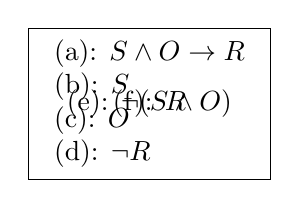
\begin{tikzpicture}
        \tikzset{level distance=60pt}
        \Tree [
            .\node[draw]{
                \begin{tabular}{l}
                    \st{(a): $S \wedge O \rightarrow R $} \\
                    (b): $S$ \\
                    (c): $O$ \\
                    (d): $\neg R$ \\
                \end{tabular}
            };
                [.\node[draw=none]{ (e): $\neg(S \wedge O)$ }; ]
                [.\node[draw=none]{ (f): $R$ }; ]
        ]
    \end{tikzpicture}
    \caption{Graph nach Expansion des Wurzelknotens}
\end{figure}

Nach Bildung des Wurzelknotens wird der Baum anhand der Tiefensuche-Traversierung expandiert. Zuerst wird der Wurzelknoten \{(a), (b), (c), (d)\}, danach der linke (e) und schliesslich der rechte Teilbaum (f) durchlaufen.

Die Transformationsregeln werden auf den Wurzelknoten angewendet. Dabei wird der linke Teilbaum (e) durch einen neu gebildeten Teilbaum (bestehend aus (g) und (h)) ersetzt, der rechte Teilbaum (f) bleibt unverändert:
\begin{enumerate}[label= (\alph*)]
    \setcounter{enumi}{6}
    \item $\neg S$
    \item $\neg O$
\end{enumerate}

\begin{figure}[htbp]
    \centering
    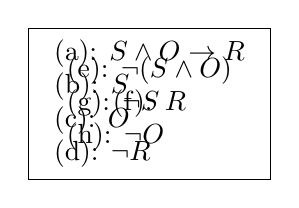
\begin{tikzpicture}
        \tikzset{level distance=60pt}
        \Tree [
            .\node[draw]{
                \begin{tabular}{l}
                    \st{(a): $S \wedge O \rightarrow R $} \\
                    (b): $S$ \\
                    (c): $O$ \\
                    (d): $\neg R$ \\
                \end{tabular}
            };
                [.\node[draw=none]{
                    \begin{tabular}{l}
                        \st{(e): $\neg(S \wedge O)$} \\
                        (g): $\neg S$\\
                        (h): $\neg O$\\
                    \end{tabular}
                };]
                [.\node[draw=none]{ (f): $R$ }; ]
        ]
    \end{tikzpicture}
    \caption{Graph nach Ersetzen der Teilbäume}
\end{figure}

Der linke Teilbaum ist somit vollständig expandiert und wird ausgewertet. Dabei werden die Knoten (b), (c), (d), (g) und (h) (logisch) vereint \textcircled{$\cup$}. Dabei ergibt sich,  dass die Knoten (g) und (h) einen Widerspruch ($\mathsf{F}$) mit den Knoten (b) und (c) bilden:
\begin{itemize}
    \item $(b) \textcircled{$\cup$} (g)$ also $S \wedge \neg S = \mathsf{F}$
    \item[] und
    \item $(c) \textcircled{$\cup$} (h)$ also $O \wedge \neg O = \mathsf{F}$
\end{itemize}

\begin{figure}[htbp]
    \centering
    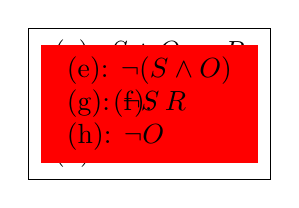
\begin{tikzpicture}
        \tikzset{level distance=60pt}
        \Tree [
            .\node[draw]{
                \begin{tabular}{l}
                    \st{(a): $S \wedge O \rightarrow R $} \\
                    (b): $S$ \\
                    (c): $O$ \\
                    (d): $\neg R$ \\
                \end{tabular}
            };
                [.\node[draw=none,fill=red]{
                    \begin{tabular}{l}
                        \st{(e): $\neg(S \wedge O)$} \\
                        (g): $\neg S$\\
                        (h): $\neg O$\\
                    \end{tabular}
                };]
                [.\node[draw=none]{ (f): $R$ }; ]
        ]
    \end{tikzpicture}
    \caption{Graph mit markiertem Teilbaum nach Widerspruch}
\end{figure}

An dieser Stelle wird die Tiefensuche im linken Unterknoten abgebrochen, dafür im rechten Unterknoten fortgesetzt. Dieser ist bereits expandiert und wird ausgewertet. Dazu muss Knoten (f) mit den Knoten (b), (c) und (d) (logisch) vereinbar sein. Auch dort herrscht ein Widerspruch:
\begin{itemize}
    \item $(d) \textcircled{$\cup$} (f)$ also $\neg R \wedge R = \mathsf{F}$
\end{itemize}

\begin{figure}[htbp]
    \centering
    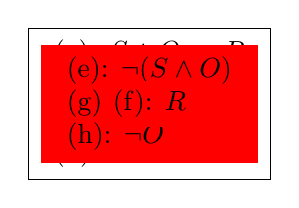
\begin{tikzpicture}
        \tikzset{level distance=60pt}
        \Tree [
            .\node[draw]{
                \begin{tabular}{l}
                    \st{(a): $S \wedge O \rightarrow R $} \\
                    (b): $S$ \\
                    (c): $O$ \\
                    (d): $\neg R$ \\
                \end{tabular}
            };
                [.\node[draw=none,fill=red]{
                    \begin{tabular}{l}
                        \st{(e): $\neg(S \wedge O)$} \\
                        (g): $\neg S$\\
                        (h): $\neg O$\\
                    \end{tabular}
                };]
                [.\node[draw=none,fill=red]{ (f): $R$ }; ]
        ]
    \end{tikzpicture}
    \caption{Graph mit markierten Teilbäumen nach Widersprüchen}
\end{figure}

Obwohl alle Knoten expandiert und ausgewertet wurden,  konnte kein Modell für $\{S \wedge O \rightarrow R, S, O, \neg R\}$ gefunden werden. Dies wiederum bedeutet, dass die \textbf{Negation} $\Gamma \models \neg\varphi$ \textbf{nicht zutrifft}. Somit \textbf{ist} $\Gamma \models \varphi$ \textbf{bewiesen}.

\subsubsection{Datentypenprüfung}
\label{ssubsection:inferenz_pellet_datatypes}
In OWL werden Datentypen in einem XML-Schema beschrieben. Dadurch sind viele einfache Datentypen wie numerische Datentypen (Ganz- und Fliesskommazahlen) und Zeichenketten gegeben. Zudem kann OWL eigene Datentypen definieren.

Das Modul zur Datentypenprüfung zeigt auf ob die Schnittmenge von Datentypen konsistent ist. Eine Schnittmenge von Datentypen ist dann inkonsistent, wenn diese keine Elemente gemeinsam haben.

Der Tableau-Reasoner nutzt dieses Modul um zu prüfen, ob die Schnittmenge aller Datentypen für jeden Literal-Knoten des Graphens erfüllbar ist.

\subsubsection{Schnittstelle zur Wissensdatenbank (KB)}
\label{ssubsection:inferenz_pellet_kb}
Die Schnittstelle zur Wissensdatenbank entscheidet, wann die Konsistenz der Abox geprüft werden muss, wann alle Konzepte neu klassifizert werden müssen und wann alle Individuen umgesetzt werden. Alle Aufgaben zum Schlussfolgern können unter geeigneter Umwandlung auf eine Prüfung der Konsistenz der Wissensdatenbank (KB) reduziert werden.

Die Schnittstelle bietet die Möglichkeit beliebige atomare Anfragen zu beantworten. Diese können Klassen, Eigenschaften oder Individuen betreffen. Wahrheitsabfragen werden in Erfüllbarkeitsprobleme umgewandelt.

Für alle Anfragen, welche mehrere Ergebnisse liefern, sind theoretisch mehrere Konsistenzprüfungen notwendig. Da dies aber sehr aufwändig ist, werden zur Optimierung im~\autoref{subsection:inferenz_pellet_opti} beschriebene Verfahren eingesetzt.

Die Schnittstelle zur Wissensdatenbank, wie auch der Rest der Komponenten von Pellet, bauen auf der ATerm-Bibliothek~\footnote{\url{https://strategoxt.org/Tools/ATermLibrary}} auf. ATerm (Annotated Term) ist ein abstratker Datentyp, welcher für den Austausch von baumartigen Datenstrukturen zwischen verteilten Applikationen entwickelt wurde.

\subsubsection{Abox Query-Engine}
\label{ssubsection:inferenz_pellet_aboxquery}
Die Schnittstelle zur Wissensdatenbank wird mit der Abox-Query-Engine verbunden. Diese beantwortet konjunktive (verknüpfte) Anfragen. Das Modul unterstützt in SPARQL oder RQDL~\footnote{\url{http://www.w3.org/Submission/RDQL/}} geschriebene Anfragen. Dabei bestehen jedoch gewisse Einschränkungen, Details siehe~\cite[S. 10 - 11]{sirin:pellet05}.

Die Abox-Query-Engine besteht im Grunde aus mehreren Query-Engines, welche Anfragen beantworten. Dabei gibt es eine zentrale Query-Engine, welche Anfragen vorverabeitet und für die Beantwortung die entsprechende Query-Engine auswählt. Details zum Ablauf, siehe~\cite[S. 11]{sirin:pellet05}.

\begin{figure}[htbp]
    \centering \rotatebox{0}{\scalebox{0.3}[0.3]{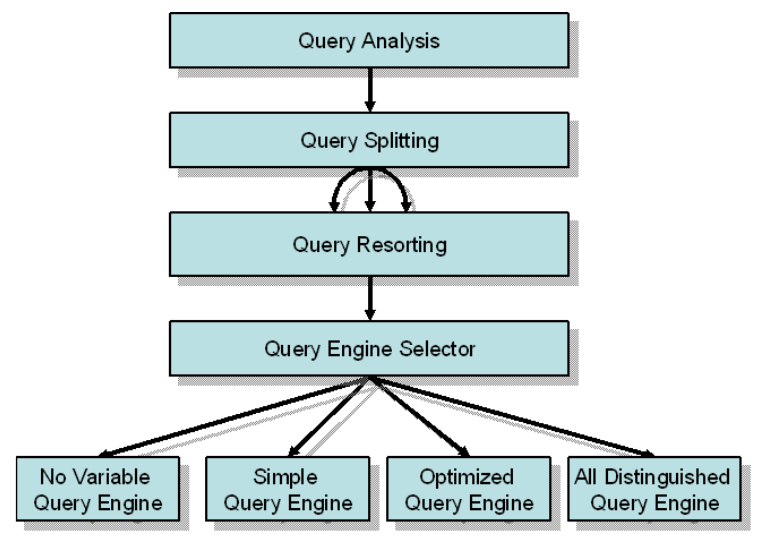
\includegraphics{bilder/infres_pellet_queryengine.png}}}
    \caption{Ablauf der Beantwortung einer Anfrage in Abox-Query-Engine.\label{fig:pellet_queryengine_komponenten}\protect\footnotemark}
\end{figure}
\footnotetext{\cite[S. 11]{sirin:pellet05}}

\subsubsection{Gültigkeitsprüfung bezüglich OWL-DL}
\label{ssubsection:inferenz_pellet_owldl}
Werkzeuge zur Modellierung und zum Export von Ontologien im OWL-Format bieten häufig Charakteristika von OWL-full zur Modellierung an. Für die Gültigkeitsprüfung einer Ontologie wird diese analysiert und gegebenenfalles mittels Heuristiken von OWL-full in OWL-DL umgewandelt.

Diese Umwandlung ist jedoch nur in gewissen Fällen möglich, so z.B.\ bei gleicher Bezeichnung von Klassen, Eigenschaften und Individuen, andernfalls werden die OWL-full Charakteristika ignoriert oder der Prozess wird abgebrochen.

\subsection{Behandlung von Regeln in Pellet}
\label{subsection:inferenz_pellet_swrl}
Pellet ermöglicht die Verwendung von Regeln zur Schlussfolgerung unter Verwendung der SWRL-Regelsprache.

Damit in der Wissensdatenbank gespeicherte Konzepte in Regeln verfügbar sind, wird das $\mathcal{AL}$-Log-Framework eingesetzt. Dieses verbindet Beschreibungslogik mit Regeln.~\cite[S. 4,5]{sirin:pellet07} $\mathcal{AL}$-Log ist ein integriertes System zur Repräsentation von Wissen, welches auf der Beschreibungslogik $\mathcal{AL}$ und der deduktiven Datenbanksprache Datalog basiert.~\cite{allog}

Bei $\mathcal{AL}$ handelt es sich um eine minimale Sprache der Beschreibungslogik, Details siehe~\cite[S. 51]{dl:baader2003}. Als Implementation des $\mathcal{AL}$-Log-Frameworks nutzt Pellet einen Datalog-Reasoner.~\cite[S. 4 - 5]{sirin:pellet07}

Bei Datalog handelt es sich um eine deklarative Logiksprache, in welcher jede Formel eine funktionsfreie Hornklausel ist. Im Unterschied zu Prolog muss jede Variable, die im Kopf einer Klausel vorkommt, auch im Körper der Klausel vorkommen. Die Reihenfolge der Klauseln spielt keine Rolle. Alle Anfragen terminieren und jede mögliche Antwort wird ausgegeben.~\cite{datalog}

In der Pellet-Implementation wird das $\mathcal{AL}$-Log-Framework dahingehend erweitert, dass es die $\mathcal{SHOIQ}(\mathcal{D})$ Variante  der $\mathcal{AL}$-Beschreibungslogik nutzen kann. Zusätzlich erlaubt die Erweiterung die Verwendung von OWL-Datentypen und SWRL-Funktionen im Körper von Datalog-Regeln.~\cite[S. 5]{sirin:pellet07}

Bei $\mathcal{SHOIQ}(\mathcal{D})$ handelt es sich um eine Erweiterung der Beschreibungslogik $\mathcal{AL}$. $\mathcal{SHOIQ}(\mathcal{D})$ unterstützt unter anderem zusätzliche Konzepte wie Rollenhierarchien, inverse Eigenschaften und qualifizierte Kardinalitätseinschränkungen. Diese Erweiterung erlaubt zusätzlich die Verwendung von Datentypen, Datenwerten und Datentypeneigenschaften.~\cite{wiki:desclog}

\subsection{Optimierungen}
\label{subsection:inferenz_pellet_opti}
Dieser Abschnitt basiert, sofern nicht anders im Text vermerkt, auf~\cite[S. 16 - 19]{sirin:pellet05}

Beschreibungslogiken, wie $\mathcal{SHOIQ}(\mathcal{D})$ haben im ungünstigsten Fall eine sehr hohe Komplexität. Daher besteht ein grosser Unterschied zwischen Design und praktischer Umsetzung einer Entscheidungsprozedur.

Um dennoch akzeptable Leistungen bei Schlussfolgerungen mittels Beschreibungslogik zu erhalten, nutzen moderne Reasoner verschiedene Arten von Optimierungen, so z.B.:

\begin{itemize}
    \item \textbf{Normalisierung und Vereinfachung}\\
        Alle Konzepte der Wissensdatenbank werden in eine Form gebracht, die hilft, Widersprüche bei der Tableau-Erweiterung möglichst früh zu erkennen. Die Konzepte werden in die Normalform gebracht.\\
        Diese Vereinfachung erkennt offensichtliche Fehler während der Normalisierung. Mehrfaches Vorkommen eines gleichen Konzeptes wird eliminiert.

    \item \textbf{Tbox-Absorption}\\
        Bei dem Prozess der Tbox-Absorption wird ebenfalls versucht, gleichartige Konzepte (GCI --- General Concept Inclusion) zu eliminieren, dies mittels Ersatz durch atomare Konzepte.

    \item \textbf{Dependency-directed Backjumping}\\
        Der Prozess des dependency-directed Backjumpings eliminiert unproduktive Backtracking-Suchen, indem er Verzweigungspunkte identifiziert welche Konflikte verursachen. Er springt zurück und überspringt dabei die Konfliktpunkte ohne nach Alternativen zu suchen.
\end{itemize}

Weitere Verfahren zur Optimierung sowie mehr Details finden sich unter~\cite[S. 17 - 19]{sirin:pellet05}.

\subsection{Unterschiede zwischen Pellet und Prolog}
\label{subsec:inferenz_pellet_prolog}
Wie unter~\ref{subsection:inferenz_pellet_swrl} erwähnt, nutzt Pellet einen Datalog-Reasoner als Implementation des $\mathcal{AL}$-Log-Frameworks.\\
Der wohl wichtigste Unterschied zu Prolog ist daher, dass in Datalog alle Anfragen terminieren und jede mögliche Antwort ausgegeben wird. Eine Reihenfolge der Klauseln spielt daher keine Rolle. Im Gegensatz dazu ist eine Termination von Anfragen in Prolog nicht immer gegeben. So sind Endlosschleifen je nach Reihenfolge der Regeln durchaus möglich.~\cite[S. 175]{laemmel}

Ein weiterer Unterschied ist die Art, wie Schlüsse gezogen werden. Prolog basiert auf dem SLD-Resolutionsverfahren~\citep[Details siehe][S. 68]{laemmel}. Im Gegensatz dazu kommt bei Pellet der unter~\ref{ssubsection:inferenz_pellet_tableaux} erklärte Tableau-Algorithmus zum Einsatz.

Durch den Aufbau von Prolog ist es möglich so genannte Constraint-Satisfaction-Probleme (Bedingungserfüllungsprobleme) zu lösen~\citep[Details siehe][S. 148]{laemmel}. Mit Pellet bzw. Ontologien und Regeln ist dies nicht der Fall. Versuche dazu finden sich den Publikationen von~\citet{xiong2008constraint},~\citet{staab2006constraint} und~\citet{bramer2007constraint}.

\noindent\rule[1ex]{\textwidth}{1pt}
\begin{wrapfigure}[15]{l}{0.1\textwidth}
    \vspace{-12pt}
    
\includegraphics[width=0.1\textwidth]{bilder/elephant.png}
\end{wrapfigure}
Das unter~\ref{ssubsection:inferenz_pellet_tableaux} genannte Beispiel beantwortet exakt die unter~\ref{sec:wissensrepFormen_Wissensnetze} gestellte Frage: Wie gelangt man zum Schluss, dass das Individuum \textit{Seilpark Balmberg} in der \textit{Region} \textit{Solothurn} liegt.

Wie gelangt man effektiv zu dieser Information? Kann diese durch reine Folgerung erreicht werden?

Die Antwort hierzu lautet ja und nein. Modelliert man die Situation beispielsweise in Protégé und unter Benützung des Pellet-Reasoners für Schlussfolgerungen, so nimmt man an, dass er dies finden kann. Aufgrund seiner Möglichkeiten sollte der Reasoner dies beantworten können. Die nachfolgende Grafik zeigt jedoch, dass dies nicht immer der Fall ist.

\begin{figure}[H]
\centering \rotatebox{0}{\scalebox{0.5}[0.5]{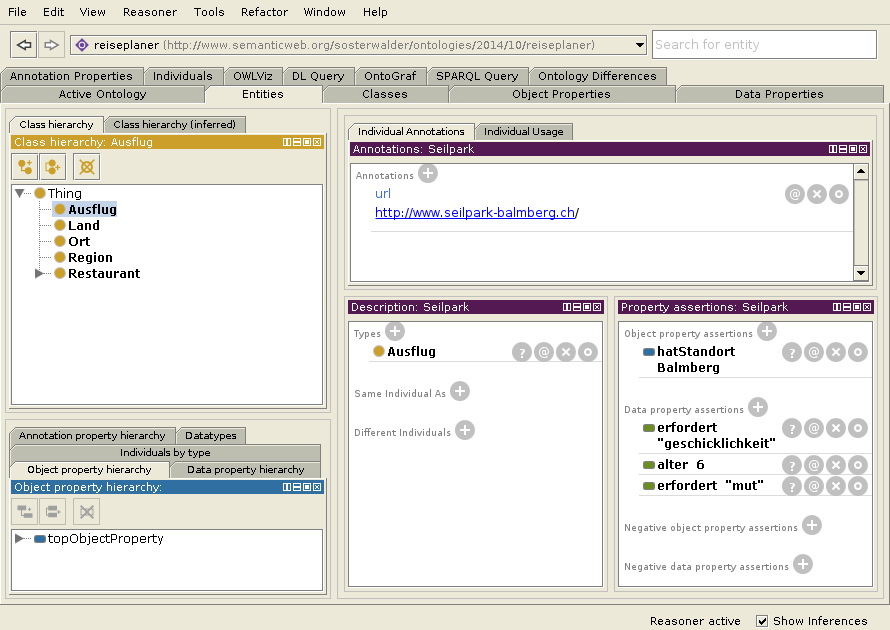
\includegraphics{bilder/inferenz_protege.png}}}
\caption{Darstellung des Individuums \textit{Seilpark Balmberg} in Protégé.\label{fig:inferenz_protege}\protect\footnotemark}
\end{figure}
\footnotetext{Eigene Darstellung mittels Stanford Protégé Version 5.0.0 beta 15}

Wenn man den Relationen die entsprechenden Eigenschaften wie Symmetrie oder Transitivität gibt, ist diese Folgerung durchaus möglich. Bei unserem Beispiel haben wir die Eigenschaften bewusst weggelassen, da andernfalls irreführende Folgerungen auftreten. So wäre z.B.\ ein Ort auch ein Land und umgekehrt.

Die eigentliche Folgerung haben wir mittels einer Regel vorgenommen. Zu einem späteren Zeitpunkt erklären wir dies genauer, siehe~\autoref{chap:swrl}.

\noindent\rule[1ex]{\textwidth}{1pt}
